\scanpage{33}\mspage{32.}
% @ top, 1°)
\deleted{\unsure{R|P|Or}} 1°) $F\setminus G\subset F'\setminus G'$ i.e. Tout $A\in F\setminus G$ est $\notin G'$. En effet, si on avait $A\in G'$, on aurait $|A|\subset|G'|=|G|$ donc \deleted{$A\in$} (comme $G\leq F$) $A\in G$.

% @ left edge, along 1°), 2°), and the following proof
% margin note written sideways; long separator rule to its right
% Approximate whole-image band of rule: x200--270, y145--1735.
\margin{\figure{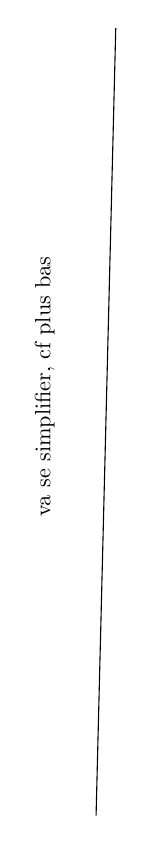
\begin{tikzpicture}[x=1cm,y=1cm]
\draw[line width=.4pt] (.65,0) -- (.90,10);
\node[rotate=90,anchor=west,scale=.8] at (0,3.7) {va se simplifier, cf plus bas};
\end{tikzpicture}}}

% @ upper middle, 2°)
2°) $F'\setminus G'\subset F\setminus G$ Soit $A'\in F'\setminus G'$, prouvons $A'\in F\setminus G$, et d'abord $A'\in F$. \deleted{On a} Soit $A$ le plus petit él. de $F^{A'}$ donc $\underline{\rule[-.15ex]{.35pt}{.55ex}\,A'\unsure{\subset|\in} A^{\deleted{\unsure{\prime|\ast|?}}},\ A'^{\circ(F')}\subset A^{\deleted{\unsure{\prime|\ast|?}}\circ(F)}\,\rule[-.15ex]{.35pt}{.55ex}}$ prouvons que $A'=A$ (d'où $A\in F$). \deleted{\unsure{On a|Or}}

% @ middle, Je dis
Je dis que $A\in F\setminus G$ i.e. $A\notin G$, sinon on aurait $A\subset|G|=|G'|$ donc $A'\in G'$ puisque $A'\in F'$ et $G'\leq F'$, absurde. \deleted{Mais} Donc $A\in F\setminus G$, donc $A\in F'$, \deleted{et} Il en résulte que $A^{\circ(F)}=A^{\circ(F')}$ (car $F'\preceq F$\inserted{il suffirait $F'\ll F$}\deleted{)} cf lemme plus bas) et \unsure{\uline{bien}|\deleted{bien}} \deleted{$\unsure{F|\in|\exists|E}$} $A,A'\in F'$ tels que $A'^{\circ(F')}\subset A^{\circ(F')}$, ce qui prouve $A=A'$.

% @ lower middle, Donc
Donc \unsure{on a} prouvé que $\deleted{\unsure{F|A}}A'\in F'\setminus G'\Rightarrow A'\in F$. Prouvons qu'on a $A'\notin G$ (d'où $A'\in F\setminus G$\deleted{)}, qed). Sinon on aurait $A'\in G$, on aurait $A'\subset |G|=|G'|$, d'où (comme $A'\in F'$ et $G'\leq F'$) $A'\in G'$, absurde.

% @ lower third, cancelled b) to c)
\deleted{b) $\Rightarrow$ c) \inserted{On suppose b) i.e. $\varphi$ induit $F'\setminus G'\overset{\sim}{\longrightarrow}F\setminus G$} Soit $A\in F\setminus G$, prouvons que $A^{\circ(F)}$ est une \uline{strate ouverte \deleted{dans \unsure{la}} de $F'$}. Soit $A'\in F'\setminus G'$ l'unique élément \deleted{de} tel que $\varphi(A')=A$.}
% The oblique cancelling strokes end above this final line; state remains open.
\unsure{Prouvons $A'^{\circ(F')}=A^{\circ(F)}$.|\deleted{Prouvons $A'^{\circ(F')}=A^{\circ(F)}$.}}

% @ bottom, b to c
b $\Longleftrightarrow$ c \deleted{Posons} On a $|F|\setminus|G|=|F'|\setminus|G'|$, soit $U$, Posons $F\setminus G=I^{\unsure{\ast|k|+}},\ F'\deleted{\unsure{\times|\setminus}}\unsure{\setminus}G'=I'^{\ast}$ (parties ouvertes des ens d'indices ordonnés $I$, \deleted{$\unsure{A|\Delta}$} $(=\unsure{F|P})$, $I'(=F')$. On a
